% !TeX root = main.tex

\documentclass[11pt]{article}
\usepackage{xltxtra}
\usepackage{bookmark}
\usepackage{hyperref}
\hypersetup{hidelinks}
\usepackage{url}
\urlstyle{tt}
\usepackage{multicol}
\usepackage{xcolor}
\usepackage{calc}
\usepackage{graphicx}
\usepackage{tikz}
\usetikzlibrary{calc}
\usepackage{fontspec}
\usepackage{xeCJK}
\usepackage{relsize}
\usepackage{xspace}
\usepackage{fontawesome5}
\usepackage{titlesec}
\usepackage{enumitem}
\usepackage{siunitx}
\usepackage{amssymb}
\usepackage{tabularx}
\usepackage{multicol}
\usepackage{fontspec}
\usepackage{fancybox}
\usepackage{float}

% ====================== 基础设置 ======================
% 取消中文字符与数字之间的间隔
\CJKsetecglue{}

% 定义美观的C++排版
\protected\def\Cpp{{C\nolinebreak[4]\hspace{-.05em}\raisebox{.28ex}{\relsize{-1}++}}\xspace}

% 全局格式设置
\setlength{\parindent}{0pt}    % 取消段落缩进
\pagenumbering{gobble}         % 取消页码显示

% 列表格式设置
\setlist[itemize]{topsep=0em, leftmargin=*}    % 项目符号列表格式
\setlist[enumerate]{topsep=0em, leftmargin=*}  % 编号列表格式

% ====================== 标题格式设置 ======================
% 一级标题格式
\titleformat{\section}
  {\LARGE\bfseries\raggedright}  % 字体：LARGE，加粗，左对齐
  {}{0em}                        % 标题前缀
  {}                             % 标题代码
  [{\color{HIT_Blue}\titlerule}]% 标题下方蓝色分隔线
\titlespacing*{\section}{0cm}{*1.2}{*1.2}  % 间距设置

% 二级标题格式  
\titleformat{\subsection}
  {\large\bfseries\raggedright}  % 字体：large，加粗，左对齐
  {}{0em}                        % 标题前缀
  {}                             % 标题代码
  []
\titlespacing*{\subsection}{0cm}{*1.2}{*1.2}  % 间距设置

% ====================== 页面布局设置 ======================
% 页面尺寸与边距
\usepackage[
    a4paper,
    left=1.2cm,
    right=1.2cm,
    top=1.5cm,
    bottom=1cm,
    nohead
]{geometry}

% 表格与正文行距设置
\renewcommand{\arraystretch}{1.2}  % 表格行距
\linespread{1.2}                   % 正文行距
\renewcommand{\CJKglue}{\hskip 0.05em}  % 中文字符间距
\emergencystretch=2em
\hfuzz=10pt
\hbadness=10000

% 带图标的节标题，同时给 PDF 书签提供纯文本标题
\newcommand{\cvsection}[2]{%
  \section[#2]{\texorpdfstring{\makebox[\widthof{#1}][c]{\color{HIT_Blue}{#1}}\quad #2}{#2}}%
}

% ====================== 字体设置 ======================
% 英文字体：狮尾四季春
\setmainfont[
  BoldFont={獅尾四季春加糖},
]{獅尾四季春加糖}

% 中文字体：狮尾四季春
\setCJKmainfont[
  BoldFont={獅尾四季春加糖},
]{獅尾四季春加糖}

% ====================== 主题色设置 ======================
% 哈工大校徽标准色（RGB: 0, 83, 117），参考https://xcb.hitwh.edu.cn/_upload/article/files/fa/5c/e1e0bdb340e98b473b5a0e34963c/6250efd5-f74a-47bb-b5a7-8a8b86f9451b.pdf第14页
\definecolor{HIT_Blue}{RGB}{0, 83, 117}

% ====================== 个人信息 ======================
% 学院信息
\newcommand{\school}{\small{电子与信息工程学院 | School of Electronics and Information Engineering}}

% 联系方式
\newcommand{\contact}{
    \scriptsize  % 使用较小字号
    \textcolor{white}{
        % 邮箱
        \faEnvelope \quad \href{mailto:23b905015@stu.hit.edu.cn}{23xxxxxx@stu.hit.edu.cn}
        \hspace{4em}
        % 手机号
        \faPhone \quad  11111111111
        % GitHub
        \hspace{4em}
        \faGithub \quad \href{https://github.com/lixb123}{https://github.com/lixb123}
    }
}

% 页面装饰
\newcommand{\cvpageforeground}{%
    \begin{tikzpicture}[remember picture, overlay]
        \node[anchor=north, inner sep=0pt](header) at (current page.north){
            \includegraphics[width=\paperwidth]{images/header.png}
        };
        \node[anchor=west](school_logo) at (header.west){
            \hspace{0.2cm}
            
\includegraphics[width=.34\textwidth]{images/hitwh_logo_name.png}
        };
        \node[anchor=east](school_name) at(header.east){
            \textcolor{white}{\textbf{\school}}
            \hspace{0.5cm}
        };
    \end{tikzpicture}

    \begin{tikzpicture}[remember picture, overlay]
        \node[anchor=south, inner sep=0pt](footer) at (current page.south){
           \includegraphics[width=\paperwidth]{images/footer.png}
        };
        \node[anchor=center] at(footer.center){\contact};
    \end{tikzpicture}%
}

\newcommand{\cvpagebackground}{%
    \begin{tikzpicture}[remember picture, overlay]
        \node[opacity=0.05] at(current page.center){
            \includegraphics[width=0.7\paperwidth, keepaspectratio]{images/hitwh_logo.png}
        };
    \end{tikzpicture}%
}

\newcommand{\cvcontinuedpagetopskip}{3em}
\newcommand{\cvpagebottomclearance}{3em}
\addtolength{\textheight}{-\cvpagebottomclearance}

%%%%%%%%%%%%%%%%%%%%
% 简历正文
%%%%%%%%%%%%%%%%%%%%
\begin{document}

\AddToHook{shipout/background}{%
    \ifnum\value{page}>1\relax
        \cvpagebackground
    \fi
}

\AddToHook{shipout/foreground}{%
    \ifnum\value{page}>1\relax
        \cvpageforeground
    \fi
}

\AddToHook{shipout/after}{%
    \ifnum\value{page}=1\relax
        \global\topskip=\cvcontinuedpagetopskip\relax
        \global\splittopskip=\cvcontinuedpagetopskip\relax
    \fi
}

% ====================== 页眉 ======================
% 包含校徽、学院名称等信息
\cvpageforeground
\vspace{-3.5em}

% ====================== 页脚 ======================
% 包含联系方式
\cvpagebackground

% ====================== 个人信息 ======================
\begin{figure}[h]
    \begin{minipage}{0.82\textwidth}
        \cvsection{\faAddressCard}{个人信息}
        \begin{tabularx}{\linewidth}{p{\widthof{出生日期:}}Xp{\widthof{政治面貌:}}X}
            姓\ \ \ \ \ \ \ \ 名: & XXX & 
            性\ \ \ \ \ \ \ \ 别: & X  \\
            出生年月: & 2XXX年X月 & 
            政治面貌: & 预备党员 \\
        \end{tabularx}
    \end{minipage}
    \hfill
    \begin{minipage}{0.12\textwidth}
        \setlength{\fboxsep}{0pt}
        \doublebox{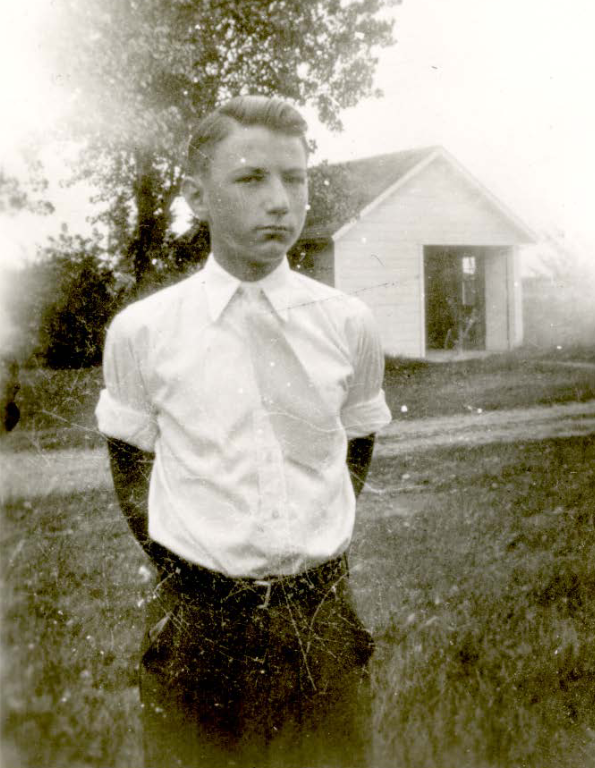
\includegraphics[width=\linewidth]{images/avatar.png}}
    \end{minipage}
\end{figure}
\vspace{-1em}

% ====================== 教育背景 ======================
\cvsection{\faGraduationCap}{教育背景}
\vspace{-0.5em}
\begin{table}[h!]
    \begin{tabularx}{\textwidth}{XXp{\widthof{2022年 -- 预计2026年6月毕业}}}
        哈尔滨工业大学 & 通信工程 & 2019年 -- 2023年6月\\
        \textbf{GPA: XX.X/100.00} & \textbf{学分绩排名: X/XX} \\
    \end{tabularx}
\end{table}
\begin{tabularx}{\textwidth}{@{}XlX@{}}
    \textbf{2023.09-2024.03} & 班级团支书 & \\
    \textbf{2024.09-2024.12} & 学生会主席 & \\
\end{tabularx}

% ====================== 项目经历 ======================
\cvsection{\faChalkboardTeacher}{在校项目}
\vspace{0.5em}
{\large{\textbf{智能图书馆管理系统}}} \hfill {进行中}\\
基于Spring Boot和Vue.js开发的图书馆管理系统，实现了图书借阅、归还、预约等功能，采用微服务架构，使用Redis缓存提高系统性能。

\vspace{1em}
{\large{\textbf{校园二手交易平台}}} \hfill {完结}\\
使用Django框架开发的校园二手交易平台，实现了用户注册、商品发布、在线交易等功能，采用RESTful API设计，使用JWT进行用户认证。

\vspace{1em}
{\large{\textbf{基于深度学习的图像分类系统}}} \hfill {完结}\\
使用PyTorch框架实现的图像分类系统，基于ResNet模型，在CIFAR-10数据集上达到了92\%的准确率，并开发了友好的Web界面。

\vspace{1em}
{\large{\textbf{智能图书馆管理系统}}} \hfill {进行中}\\
基于Spring Boot和Vue.js开发的图书馆管理系统，实现了图书借阅、归还、预约等功能，采用微服务架构，使用Redis缓存提高系统性能。

\vspace{1em}
{\large{\textbf{校园二手交易平台}}} \hfill {完结}\\
使用Django框架开发的校园二手交易平台，实现了用户注册、商品发布、在线交易等功能，采用RESTful API设计，使用JWT进行用户认证。

\vspace{1em}
{\large{\textbf{基于深度学习的图像分类系统}}} \hfill {完结}\\
使用PyTorch框架实现的图像分类系统，基于ResNet模型，在CIFAR-10数据集上达到了92\%的准确率，并开发了友好的Web界面。

\vspace{1em}
{\large{\textbf{智能图书馆管理系统}}} \hfill {进行中}\\
基于Spring Boot和Vue.js开发的图书馆管理系统，实现了图书借阅、归还、预约等功能，采用微服务架构，使用Redis缓存提高系统性能。

\vspace{1em}
{\large{\textbf{校园二手交易平台}}} \hfill {完结}\\
使用Django框架开发的校园二手交易平台，实现了用户注册、商品发布、在线交易等功能，采用RESTful API设计，使用JWT进行用户认证。

\vspace{1em}
{\large{\textbf{基于深度学习的图像分类系统}}} \hfill {完结}\\
使用PyTorch框架实现的图像分类系统，基于ResNet模型，在CIFAR-10数据集上达到了92\%的准确率，并开发了友好的Web界面。

\vspace{1em}
{\large{\textbf{智能图书馆管理系统}}} \hfill {进行中}\\
基于Spring Boot和Vue.js开发的图书馆管理系统，实现了图书借阅、归还、预约等功能，采用微服务架构，使用Redis缓存提高系统性能。

\vspace{1em}
{\large{\textbf{校园二手交易平台}}} \hfill {完结}\\
使用Django框架开发的校园二手交易平台，实现了用户注册、商品发布、在线交易等功能，采用RESTful API设计，使用JWT进行用户认证。

\vspace{1em}
{\large{\textbf{基于深度学习的图像分类系统}}} \hfill {完结}\\
使用PyTorch框架实现的图像分类系统，基于ResNet模型，在CIFAR-10数据集上达到了92\%的准确率，并开发了友好的Web界面。

% ====================== 竞赛经历 ======================
\cvsection{\faTrophy}{竞赛经历}
\vspace{-1em}
\begin{table}[h!]
    \begin{tabularx}{\textwidth}{Xp{\widthof{第零零负责人人人}}p{\widthof{国家级-第100名}}p{\widthof{2030年13月}}}
        \textbf{2023年全国大学生数学建模竞赛} & 队长 & 全国一等奖 & 2023年9月 \\
        \textbf{2023年"互联网+"大学生创新创业大赛} & 核心成员 & 省级金奖 & 2023年7月\\
        \textbf{2023年ACM-ICPC亚洲区域赛} & 队员 & 铜奖 & 2023年11月\\
        \textbf{2023年全国大学生数学建模竞赛} & 队长 & 全国一等奖 & 2023年9月 \\
        \textbf{2023年"互联网+"大学生创新创业大赛} & 核心成员 & 省级金奖 & 2023年7月\\
        \textbf{2023年ACM-ICPC亚洲区域赛} & 队员 & 铜奖 & 2023年11月\\
    \end{tabularx}
\end{table}

% ====================== 技能特长 ======================
\cvsection{\faWrench}{技能特长}
\vspace{0.5em}
\begin{itemize}
    \item 编程语言：熟练掌握Java、Python、C++，了解Go、Rust
    \item Web开发：熟悉Spring Boot、Django、Vue.js等框架
    \item 数据库：熟练使用MySQL、Redis、MongoDB
\end{itemize}

% ====================== 所获荣誉 ======================
\cvsection{\faStar}{所获荣誉}
\vspace{-1em}
\begin{multicols}{2}
    \begin{itemize}
        \item 2022-2023学年一等奖学金
        \item 2022-2023学年校级优秀学生干部
    \end{itemize}
\end{multicols}

\end{document}
